% AxBi Modular System Interface Map — TikZ source
% Compile with pdflatex + tikz; or use the SVG export in docs/assets/axbi-system-architecture.svg

\begin{figure}[H]
\centering
\fitwidth{%
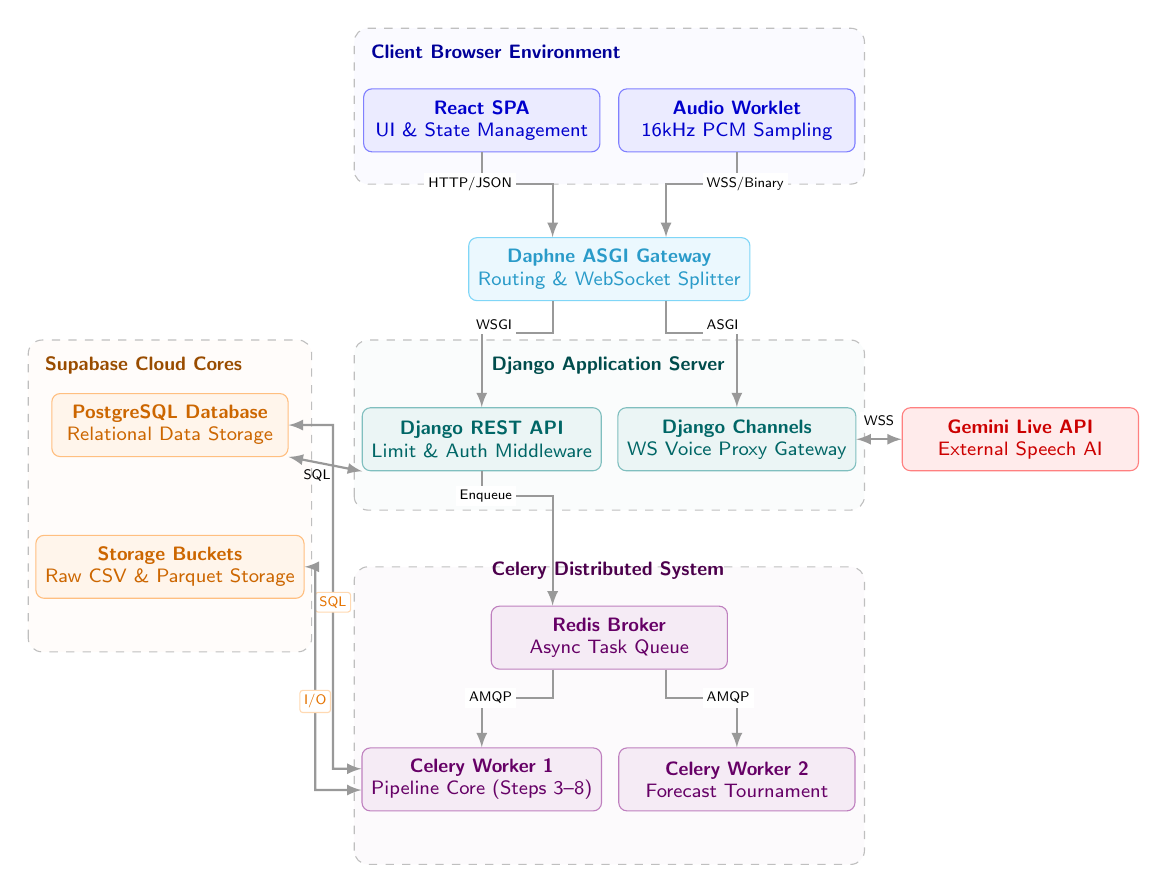
\begin{tikzpicture}[
    xscale=0.9, yscale=0.9,
    node distance=1.2cm and 1.5cm,
    box/.style={rectangle, draw, rounded corners=3pt, minimum width=3.0cm, minimum height=0.8cm, align=center, font=\scriptsize\sffamily},
    arrow/.style={-latex, thick, draw=gray!80, font=\tiny\sffamily},
    doublearrow/.style={latex-latex, thick, draw=gray!80, font=\tiny\sffamily},
    client/.style={box, fill=blue!8, draw=blue!50, text=blue!80!black},
    gateway/.style={box, fill=cyan!8, draw=cyan!50, text=cyan!80!black},
    django/.style={box, fill=teal!8, draw=teal!50, text=teal!80!black},
    db/.style={box, fill=orange!8, draw=orange!50, text=orange!80!black},
    celery/.style={box, fill=violet!8, draw=violet!50, text=violet!80!black}
]
    \draw[dashed, gray!50, fill=blue!2!white, rounded corners=5pt] (4.2, 7.0) rectangle (11.4, 9.2);
    \node[anchor=north west, font=\scriptsize\bfseries\sffamily, text=blue!60!black] at (4.3, 9.1) {Client Browser Environment};

    \draw[dashed, gray!50, fill=orange!2!white, rounded corners=5pt] (-0.4, 0.4) rectangle (3.6, 4.8);
    \node[anchor=north west, font=\scriptsize\bfseries\sffamily, text=orange!60!black] at (-0.3, 4.7) {Supabase Cloud Cores};

    \draw[dashed, gray!50, fill=teal!2!white, rounded corners=5pt] (4.2, 2.4) rectangle (11.4, 4.8);
    \node[anchor=north west, font=\scriptsize\bfseries\sffamily, text=teal!60!black] at (6, 4.7) {Django Application Server};

    \draw[dashed, gray!50, fill=violet!2!white, rounded corners=5pt] (4.2, -2.6) rectangle (11.4, 1.6);
    \node[anchor=north west, font=\scriptsize\bfseries\sffamily, text=violet!60!black] at (6, 1.8) {Celery Distributed System};

    \node (react) at (6.0, 7.9) [client] {\textbf{React SPA} \\ UI \& State Management};
    \node (worklet) at (9.6, 7.9) [client] {\textbf{Audio Worklet} \\ 16kHz PCM Sampling};

    \node (daphne) at (7.8, 5.8) [gateway] {\textbf{Daphne ASGI Gateway} \\ Routing \& WebSocket Splitter};

    \node (drf) at (6.0, 3.4) [django] {\textbf{Django REST API} \\ Limit \& Auth Middleware};
    \node (channels) at (9.6, 3.4) [django] {\textbf{Django Channels} \\ WS Voice Proxy Gateway};

    \node (db) at (1.6, 3.6) [db] {\textbf{PostgreSQL Database} \\ Relational Data Storage};
    \node (storage) at (1.6, 1.6) [db] {\textbf{Storage Buckets} \\ Raw CSV \& Parquet Storage};

    \node (gemini) at (13.6, 3.4) [box, fill=red!8, draw=red!50, text=red!80!black] {\textbf{Gemini Live API} \\ External Speech AI};

    \node (redis) at (7.8, 0.6) [celery] {\textbf{Redis Broker} \\ Async Task Queue};
    \node (worker1) at (6.0, -1.4) [celery] {\textbf{Celery Worker 1} \\ Pipeline Core (Steps 3--8)};
    \node (worker2) at (9.6, -1.4) [celery] {\textbf{Celery Worker 2} \\ Forecast Tournament};

    \draw[arrow] (react.south) -- ++(0,-0.45) -| ([xshift=-0.8cm]daphne.north) node[pos=0.25, left, fill=white, inner sep=1.5pt] {HTTP/JSON};
    \draw[arrow] (worklet.south) -- ++(0,-0.45) -| ([xshift=0.8cm]daphne.north) node[pos=0.25, right, fill=white, inner sep=1.5pt] {WSS/Binary};

    \draw[arrow] ([xshift=-0.8cm]daphne.south) -- ++(0,-0.45) -| (drf.north) node[pos=0.25, left, fill=white, inner sep=1.5pt,yshift=3pt] {WSGI};
    \draw[arrow] ([xshift=0.8cm]daphne.south) -- ++(0,-0.45) -| (channels.north) node[pos=0.25, right, fill=white, inner sep=1.5pt,yshift=3pt] {ASGI};

    \draw[doublearrow] (channels.east) -- (gemini.west) node[midway, above, fill=white, inner sep=1.5pt, yshift=3pt] {WSS};

    \draw[doublearrow] (drf.195) -- (db.345) node[pos=0.5, above,xshift=-3pt ,yshift=-8pt, inner sep=1.5pt] {SQL};

    \draw[arrow] (drf.south) -- ++(0,-0.35) -| ([xshift=-0.8cm]redis.north) node[pos=0.25, left, fill=white, inner sep=1.5pt] {Enqueue};

    \draw[arrow] ([xshift=-0.8cm]redis.south) -- ++(0,-0.4) -| (worker1.north) node[pos=0.25, left, fill=white, inner sep=1.5pt] {AMQP};
    \draw[arrow] ([xshift=0.8cm]redis.south) -- ++(0,-0.4) -| (worker2.north) node[pos=0.25, right, fill=white, inner sep=1.5pt] {AMQP};

    \draw[doublearrow] ([yshift=0.15cm]worker1.west) -- (3.9, -1.25) |- (db.east);
    \node[fill=white, inner sep=1.5pt, font=\tiny\sffamily, text=orange!90!black, draw=orange!30, rounded corners=1pt] at (3.9, 1.1) {SQL};

    \draw[doublearrow] ([yshift=-0.15cm]worker1.west) -- (3.65, -1.55) |- (storage.east);
    \node[fill=white, inner sep=1.5pt, font=\tiny\sffamily, text=orange!90!black, draw=orange!30, rounded corners=1pt] at (3.65, -0.3) {I/O};

\end{tikzpicture}%
}
\caption{AxBi Modular System Interface Map}
\label{fig:system_arch_map}
\end{figure}
